% This is samplepaper.tex, a sample chapter demonstrating the
% LLNCS macro package for Springer Computer Science proceedings;
% Version 2.20 of 2017/10/04
%
\documentclass[runningheads]{llncs}
%
\usepackage{graphicx}
% Used for displaying a sample figure. If possible, figure files should
% be included in EPS format.
%
% If you use the hyperref package, please uncomment the following line
% to display URLs in blue roman font according to Springer's eBook style:
% \renewcommand\UrlFont{\color{blue}\rmfamily}

\begin{document}
%
\title{Admission Handler}

\author{Group 18: Jan Haas \and Simon Hauser \and Sam Kenworthy}

\institute{}
%
\maketitle              % typeset the header of the contribution

\section{Introduction}
This project implements a distributed admission system for large events and venues with limited capacity.
The stream of visitors entering or exiting the venue will be monitored in real-time via mobile devices at each entrance.
Live feedback will be provided to each device, enabling organizers to stop admission when the maximum capacity of the venue has been reached.

%(Extended) As the world starts to reopen after the pandemic and public events become possible again, systems are required to handle the keeping of safe capacities, in-line with changing guidelines and laws. Pre-selling tickets is one possibility of managing these limits, yet events such as Christmas markets, beer gardens and public concerts live off spontaneous visits. This project will enable the simple monitoring and managing of such streams of visitors, by providing a dynamically scalable system by using end-user mobile devices as client-hosts.
\section{Requirements Analysis}

\begin{itemize}
    \item [Dynamic discovery:] In case of a surge of guests to the venue, additional devices must be able to join the system without changing the current count and obtain the current state of the system. Causal ordering of messages is required to ensure that visitors are admitted in the correct order.
    \item [Leader election:] New devices must be authorized to join the system.
    \item [Reliable ordered multicast:] All devices must be able to display the current count of people inside the venue. The order of value increments must be reliable to prevent overstepping the maximum capacity. Messages may not get lost as this would mean unaccounted visitors.
    \item [Fault tolerance:] The failure or disconnection of a client component should not influence the system. System components must be redundant to prevent the loss of data.
\end{itemize}
\section{Architecture}
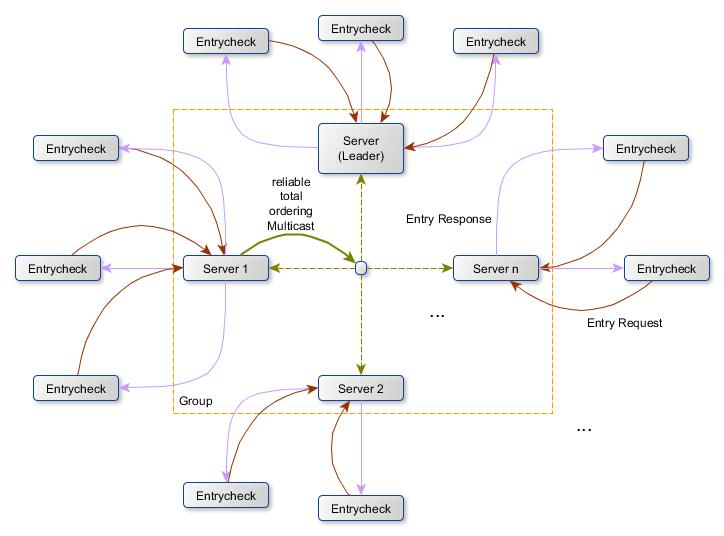
\includegraphics[width=\textwidth]{architecture_graph.jpg}

\end{document}
